\documentclass{beamer}
\usefonttheme{professionalfonts}
\usepackage{xeCJK}
\usepackage{bm}
\usepackage{amsmath}
\usepackage{amssymb}
\usepackage{graphicx}
\usepackage{appendix}
\usepackage{ulem}
\usepackage{cancel}
\usepackage{animate}
\usepackage{subfigure}
\usepackage{color}
\usepackage{amsthm}
\usepackage{hyperref}
\usepackage{algorithm}
\usepackage{algorithmic}
\setCJKmainfont[BoldFont=SimHei,ItalicFont={[stkaiti.ttf]}]{SimSun}
\newtheorem{thm}{定理}[section]
\newtheorem{defn}[thm]{定义}
\newtheorem{rela}[thm]{关系}
%\newtheorem{mydefinition}{\heiti 定义}[section]
%\newtheorem{mytheorem}[mydefinition]{\heiti 定理}
%\newtheorem{myproposition}[mydefinition]{\heiti 命题}
%\newtheorem{mylemma}[mydefinition]{\heiti 引理}
%\newtheorem{mycorollary}[mydefinition]{\heiti 推论}
\usetheme{CambridgeUS}
\begin{document}
%%-------------------------------------------------
    \title{基本优化方法(现学现卖)}
    \author{李显求}
    \institute{VIPL Group}
    \date{\today}
    \frame{\titlepage}
%%-------------------------------------------------
%%------------Frame 01-----------------------------
\begin{frame}\frametitle{提纲}
\begin{itemize}
\item 主要内容
\begin{itemize}
\item 凸问题
\item 泰勒展开式%\ref{Taylor_Externtion}
\item 梯度下降法%\ref{Gradient_Descend_Method}
\item 牛顿迭代法%\ref{Newton_Method}
\item Levenberg–Marquardt算法%\ref{LM_Method}
\item 拟牛顿法%\ref{BFGS_Method}
\begin{itemize}
\item BFGS算法%\ref{BFGS_Method}
\item L-BFGS算法%\ref{LBFGS_Method}
\end{itemize}
\item 次梯度算法%\ref{SubGradient_Method}
\item Bregman Projection Problem及解法%\ref{Bregman_Projection}
\item Lagrange 对偶问题%\ref{Lagrange_Dual_Problem}
\item 几个例子%\ref{Examples}
\end{itemize}
\item Q\&A
\end{itemize}
\end{frame}
%%------------Frame 1.5-----------------------------
\begin{frame}\frametitle{符号编辑页1(相当于草稿)}
\begin{itemize}
\item 凸集合$\bm{x}_1,\bm{x}_2 \in S,\textbf{then } \bm{x}=\lambda \bm{x}_1+(1-\lambda)\bm{x}_2 \in S$
\item 凸函数$f(\lambda \bm{x}_1+(1-\lambda)\bm{x}_2)=f(\bm{x}_2+\lambda(\bm{x}_1-\bm{x}_2))<\lambda f(\bm{x}_1)+(1-\lambda)f(\bm{x}_2),\lambda \in (0,1)$
\item Bregman Divergence:$D_{F}(\bm{p},\bm{q})=F(\bm{p})-F(\bm{q})-\left<\nabla F(q),\bm{p}-\bm{q}\right>$
\item $f$是一个线性函数和一个常数的和,也就是$f(\bm{x})=A\bm{x}+\bm{b}$的形式,其中$A\in R^{m\times n},\bm{b} \in R^m$,那么$f:R^n\rightarrow R^m$是仿射的
\item 逐点上确界$g(\bm{x})=\sup \{f_{1}(\bm{x}),f_{2}(\bm{x}),\cdots\}$
\item $\mathcal{L}(x,\lambda)=f_1(x)+\lambda f_{0}(x)$
\item $s(x)=\frac{\exp(x)}{1+\exp(x)}=\frac{1}{1+\exp(-x)},s^{\prime}(x)=s(x)(1-s(x))$
\item $\min |x|,t_i=\frac{1}{i+1}$
\item ${\rm dist}^{2}_{x^{\prime}\in S}(x^{\prime},x),S$
\begin{equation}
\left\{
\begin{split}
&\min f_1(x)\\
&f_{0}(x)<0
\end{split}
\right.
\end{equation}
\end{itemize}
\end{frame}
%%------------Frame 1.7-----------------------------
\begin{frame}\frametitle{符号编辑页2(相当于草稿)}
\begin{itemize}
\item $D_{ld}(A,A_0)={\rm tr}(AA_{0}^{-1})-\log{\rm det}(AA_{0}^{-1})-n$
\item $F(X)=-\log|{\rm det}(X)|,\nabla_{X}F(X)=-(X^{T})^{-1}$
\begin{equation}
\begin{split}
&\min_{A\succeq 0}D_{ld}(A,A_0)+\gamma D_{ld}({\rm diag}(\xi),{\rm diag}(\xi_0))\\
s.t~~&{\rm tr}(A(x_{i}-x_{j})(x_{i}-x_{j})^{T})\leq \xi_{ij},(i,j)\in S\\
&{\rm tr}(A(x_{i}-x_{j})(x_{i}-x_{j})^{T})\geq \xi_{ij},(i,j)\in D\\
\end{split}
\end{equation}
\begin{equation}
\begin{split}
&\min_{A\succeq 0}D_{ld}(A_{k+1},A_{k})+\gamma D_{ld}({\rm diag}(\xi_{k+1}),{\rm diag}(\xi_k))\\
&s.t~~\delta_{ij}{\rm tr}(A_{k+1}(x_{i}-x_{j})(x_{i}-x_{j})^{T})\leq \delta_{ij}\xi_{ij}\\
&~~~~~~~~~~~~~\delta_{ij}=\left\{
\begin{split}
&1,~if~ (i,j)\in S\\
&-1,~if~ (i,j)\in D\\
\end{split}
\right.
\end{split}
\end{equation}
\end{itemize}
\end{frame}
%%------------Frame 1.9-----------------------------
\begin{frame}\frametitle{符号编辑页3(相当于草稿)}
\begin{itemize}
\item $D_{ld}(A,A_0)={\rm tr}(AA_{0}^{-1})-\log{\rm det}(AA_{0}^{-1})-n$
\item $F(X)=-\log|{\rm det}(X)|,\nabla_{X}F(X)=-(X^{T})^{-1}$
\begin{equation}
\begin{split}
\mathcal{L}(A,\beta)&=D_{ld}(A,A_k)+\gamma D_{ld}({\rm diag}(\xi_{k+1}),{\rm diag}(\xi_k))\\
&+\alpha(\delta_{ij}{\rm tr}(A(\bm{x}_{i}-\bm{x}_{j})(\bm{x}_{i}-\bm{x}_{j})^{T})-\delta_{ij}\xi_{ij})\\
\nabla_{A}\mathcal{L}(A,\beta)&=(A_{k}^{-1})^{T}-(A^{-1})^{T}+\alpha \delta_{ij}C_{ij}^{T}\\
A&=(A_{k}^{-1}+\alpha \delta_{ij}C_{ij})^{-1}\\
&=A_{k}-\alpha\delta_{ij}\frac{A_{k}(\bm{x}_i-\bm{x}_j)(\bm{x}_i-\bm{x}_j)^{T}A_{k}}{1+\alpha\delta_{ij}(\bm{x}_i-\bm{x}_j)A_{k}(\bm{x}_i-\bm{x}_j)}
\end{split}
\end{equation}
\begin{equation}
\begin{split}
D\log{\rm det}(AB)(A)[H]&=D\log{\rm det}(AB)(AB)[D(AB)(A)[H]]\\
&=D\log{\rm det}(AB)(AB)[HB]\\
&=\left<\nabla_{AB}\log{\rm det}(AB),(HB)^{T}\right>\\
&=\left<((AB)^{-1})^{T},(HB)^{T}\right>\\
&={\rm tr}((A^{-1})^{T}(B^{-1})^{T}B^{T}H^{T})\\
&=\left<(A^{-1})^{T},H \right>
\end{split}
\end{equation}
\end{itemize}
\end{frame}
%%------------Frame 1.9.9-----------------------------
\begin{frame}\frametitle{符号编辑页3(相当于草稿)}
\begin{itemize}
\item   
\begin{equation}
\begin{split}
\nabla_{A_{k+1}}D_{ld}(A_{k+1},A_0)&=\nabla_{A_{k}}D_{ld}(A_{k},A_0)+\alpha \delta_{ij}C_{ij}\\
(A_{0}^{-1})^{T}-(A_{k+1}^{-1})^{T}&=(A_{0}^{-1})^{T}-(A_{k}^{-1})^{T}+\alpha \delta_{ij}C_{ij}\\
A_{k+1}&=(A_{k}^{-1}-\alpha \delta_{ij}C_{ij})^{-1}\\
&=A_{k}+\alpha\delta_{ij}\frac{A_{k}(\bm{x}_i-\bm{x}_j)(\bm{x}_i-\bm{x}_j)^{T}A_{k}}{1-\alpha\delta_{ij}(\bm{x}_i-\bm{x}_j)A_{k}(\bm{x}_i-\bm{x}_j)}
\end{split}
\end{equation}
\end{itemize}
\end{frame}
%%------------Frame 02-----------------------------
\begin{frame}\frametitle{从泰勒展开说起}
\label{Taylor_Externtion}
\begin{defn}
设$f(x)$是实数域上的无穷可微的函数,那么它在任意一点$x_0$泰勒展开式表示为\footnote{这里只讨论优化问题故省略了关于收敛域的讨论;所以只需要知道它是$x_0$周围的一个小领域就可以了,优化时只要步长不太大一般不会违反这个准则}:
\begin{equation}
\label{Taylor_Extention_1}
f(x)=f(x_0)+f'(x_0)(x-x_0)+\frac{f''(x_0)}{2!}(x-x_0)^2+\cdots
\end{equation}
同样的对于无穷可微向量函数$f(\bm{x})$以及初始点$\bm{x_0}$有\footnote{其中$\bm{H}$矩阵就是通常意义的Hessian矩阵}:
\begin{equation}
\label{Taylor_Extention_d}
f(\bm{x})=f(\bm{x_0})+\left(\frac{\partial f(\bm{x_0})}{\partial \bm{x}}\right)^{T}(\bm{x-x_0})+\frac{1}{2!}(\bm{x-x_0})^{T}\bm{H}(\bm{x-x_0})+\cdots
\end{equation}
\end{defn}
\end{frame}
%%------------Frame 03-----------------------------
\begin{frame}\frametitle{梯度下降优化方法}
\label{Gradient_Descend_Method}
首先,梯度下降涉及两个参数:方向$\bm{g}$和步长$\alpha$,为了方便起见这里不妨假设$\|\bm{g}\|=1$(虽然在实际中我们并不一定做归一化)。\\
最优化的目的就是使得$f(\bm{x_0}+\alpha \bm{g})$最小,于是利用一阶泰勒展开我们得到:
\begin{equation}
\label{Gradient_Descend}
f(\bm{x_0}+\alpha \bm{g}) \approx f(\bm{x_0})+\alpha\left(\frac{\partial f(\bm{x_0})}{\partial \bm{x}}\right)^{T}\bm{g}
\end{equation}
上式右边当$\bm{g}=-\left(\frac{\partial f(\bm{x_0})}{\partial \bm{x}}\right)/\|\frac{\partial f(\bm{x_0})}{\partial \bm{x}}\|$的时候是$f(\bm{x_0}+\alpha \bm{g})$较$f(\bm{x_0})$下降最快的方向,所以梯度下法也叫最速下降法。\\
至于步长$\alpha$的选择则是一个一维的优化问题,这个问题比较简单(二分法,0.618法等都可以解决),当然也可以是预先定义的。\\
对于凸函数由于有:$f(\bm{x})\geq f(\bm{x_0})+\left(\frac{\partial f(\bm{x_0})}{\partial \bm{x}}\right)^{T}(\bm{x-x_0})$,所以梯度下降算法可以保证目标函数值是不增加的
\end{frame}
%%------------Frame 04-----------------------------
\begin{frame}\frametitle{牛顿迭代法(1/3)}
\label{Newton_Method}
下面的动画显示了牛顿法在一维时的情况,这也相当于阐述了牛顿法的几何意义\\
\vspace{-3mm}
\begin{center}
\animategraphics[autoplay,loop,controls,buttonsize=3mm, height=0.6\textheight]{1}{NewtonIteration_Ani/}{1}{17}
\end{center}
在下一页中将使用数学来解释这种过程了,也就是牛顿法(牛顿迭代)的数学形式。
\end{frame}
%%------------Frame 05-----------------------------
\begin{frame}\frametitle{牛顿迭代法(2/3)}
类似于梯度下降算法,首先给出$f(x)$的二阶泰勒展开式\footnote{\color{red}需要注意的是:牛顿法计算的是零点(或者说方程的根,因此,其实牛顿法是通过极值点处的梯度为零将两者联系起来}
\begin{equation}
\label{Newton_Method_Taylor}
\begin{split}
&f(\bm{x})=f(\bm{x_0})+\left(\frac{\partial f(\bm{x_0})}{\partial \bm{x}}\right)^{T}(\bm{x-x_0})+\frac{1}{2!}(\bm{x-x_0})^{T}\bm{H}(\bm{x-x_0})+\cdots\\
&\frac{\partial f(\bm{x})}{\partial \bm{x}}=\frac{\partial f(\bm{x_0})}{\partial \bm{x}}+\bm{H}(\bm{x-x_0})+\cdots\\
\end{split}
\end{equation}
不难发现的是过$\bm{x_0}$点$\frac{\partial f(\bm{x})}{\partial \bm{x}}$的"切平面"的就是:
\begin{equation}
\label{Newton_Method_Tangent}
\bm{y}=\frac{\partial f(\bm{x_0})}{\partial \bm{x}}+\bm{H}(\bm{x-x_0})
\end{equation}
\end{frame}
%%------------Frame 06-----------------------------
\begin{frame}\frametitle{牛顿迭代法(3/3)}
在公式$\bm{y}=\frac{\partial f(\bm{x_0})}{\partial \bm{x}}+\bm{H}(\bm{x-x_0})$中,令$\bm{y=0}$可以得到:
\begin{equation}
\label{Newton_Method}
\begin{split}
&\bm{x}=\bm{x_0}-\bm{H^{-1}}\frac{\partial f(\bm{x_0})}{\partial \bm{x}}\\
&~~~~~~~~~~~or\\
&\bm{x_{k+1}}=\bm{x_k}-\bm{H^{-1}}\frac{\partial f(\bm{x_k})}{\partial \bm{x}}\\
\end{split}
\end{equation}
在最后,这里在举一个例子用来说明牛顿法的应用(求一个实数$a$的$n$次方根):
\begin{itemize}
\item 首先写出方程:$f(x)=x^{n}-a$,则$f(x)$的零点即为所求。
\item 根据牛顿迭代法得到更新公式:$x_{k+1}=x_{k}-\frac{x_{k}^{n}-a}{nx_{k}^{n-1}}$。
\item 最后由于算法是二阶的所以很快就会收敛了。
\end{itemize}
\end{frame}
%%------------Frame 07-----------------------------
\begin{frame}\frametitle{Levenberg–Marquardt算法}
\label{LM_Method}
假设$f$是一个从$\mathbb{R}^m \rightarrow \mathbb{R}^n$的非线性映射,也就是说$\bm{x} \in \mathbb{R}^m$,经过$f$变换$\bm{y}=f(\bm{w}|\bm{x})$有$\bm{y} \in \mathbb{R}^{n}$。

Levenberg–Marquardt算法的目的就是希望任意给定一个$\bm{y}$以及合理的初始值$\bm{w_0}$,能找到一个 $\bm{w^*}$,使得$\bm{\epsilon}^T\bm{\epsilon}$尽量小(局部极小),其中$\bm{\epsilon}=f(\bm{w^*}|\bm{x})-\bm{y}$

接着还是请出$f(\bm{w}|\bm{x})$的泰勒展开(一阶):$f(\bm{w}+\bm{g})\approx f(\bm{w}|\bm{x})+\bm{J}\bm{g}$
对于第$k+1$次迭代:
\begin{equation}
\label{Levmar_obj}
\begin{split}
\min \|\bm{\epsilon_{k+1}}\|^{2}&=\min \|\bm{y}-f(\bm{w}+\bm{g}_k)\|\\
&\approx \min \|\bm{y}-f(\bm{w}|\bm{x})-\bm{Jg_k}\|^2\\
&=\min \|\bm{\epsilon_{k}}-\bm{Jg_k}\|\\
\end{split}
\end{equation}
该最小二乘问题有解析解:$(\bm{J^{T}J})\bm{g_k}=\bm{J}^{T}\bm{\epsilon_{k}}$\\
对该式稍作修改可以得到(类似于岭回归):$(\mu\bm{I}+\bm{J^{T}J})\bm{g_k}=\bm{J}^{T}\bm{\epsilon_{k}}$\\
最后再说一句:当$\mu$较大的时候上式接近梯度下降,反之接近牛顿法
\end{frame}
%%------------Frame 08-----------------------------
\begin{frame}\frametitle{BFGS算法(1/2)}
\label{BFGS_Method}
BFGS(\textbf{B}royden,\textbf{F}letcher,\textbf{G}oldfarb,\textbf{S}hanno);本节内容参考:\url{http://blog.csdn.net/itplus/article/details/21896453}

牛顿法是二阶收敛的,速度上是非常理想的;但是Hessian矩阵非常难以计算,在实际计算中往往得不偿失甚至计算不出来;\textbf{拟牛顿法}应运而生,其核心就是如何估计Hessian矩阵(或其逆)。\\
另一方面为了判断估计的好坏,于是有了\textbf{拟牛顿条件},首先回顾牛顿法中的公式:
\begin{displaymath}
\frac{\partial f(\bm{x})}{\partial \bm{x}}\approx \frac{\partial f(\bm{x_0})}{\partial \bm{x}}+\bm{H}(\bm{x-x_0})
\end{displaymath}
令$x=x_{k+1},x_0=x_k$并令$\bm{g_{k+1}}=\frac{\partial f(\bm{x_{k+1}})}{\partial \bm{x}},\bm{g_{k}}=\frac{\partial f(\bm{x_{k}})}{\partial \bm{x}}$带入上式得到\textbf{拟牛顿条件}:
\begin{displaymath}
\bm{g_{k+1}-g_k}\approx \bm{H}_k(\bm{x_{k+1}-x_k})
\end{displaymath}
最后$\bm{s_k}\triangleq \bm{x_{k+1}-x_k},\bm{y_k}\triangleq \bm{g_{k+1}-g_k}$带入得到:
\begin{displaymath}
\bm{s_k}\approx \bm{H}^{-1}\bm{y_k}~or~\bm{y_k}\approx \bm{H}\bm{s_k}
\end{displaymath}
\end{frame}
%%------------Frame 09-----------------------------
\begin{frame}\frametitle{BFGS算法(2/2)}
{\color{red}与DFP\footnote{\url{http://blog.csdn.net/itplus/article/details/21896981}}不同BFGS算法估计的是Hessian矩阵而前者估计的是Hessian矩阵的逆}

BFGS:利用迭代式$\bm{B}_{k+1}=\bm{B}_k+\Delta \bm{B}_k$估计$\bm{H}_k$:$\bm{B}_{k+1}\approx \bm{H}_k$,其主要有以下几步:
\begin{itemize}
\item 假设$\Delta\bm{B}_k=\alpha \bm{uu}^{T}+\beta \bm{vv}^{T}$,其中$\alpha,\beta,\bm{u},\bm{v}$待定
\item 带入拟牛顿条件:$\bm{y_k}\approx \bm{B}_k\bm{s}_k+(\alpha \bm{uu}^{T}+\beta \bm{vv}^{T})\bm{s_k}=\bm{B}_k\bm{s}_k+(\alpha \bm{u}^{T}\bm{s_k})\bm{u}+(\beta \bm{v}^{T}\bm{s_k})\bm{v}$。
\item 令$(\alpha \bm{u}^{T}\bm{s_k})=1,(\beta \bm{v}^{T}\bm{s_k})=-1,\bm{u}=\bm{y}_k,\bm{v}=\bm{B}_k\bm{s}_k$。
\item 解得$\alpha=\frac{1}{\bm{y}_{k}^{T}\bm{s}_k},\beta=\frac{1}{\bm{s}_{k}^{T}\bm{B}_{k}\bm{s}_k}$,于是$\Delta \bm{B}_k=\frac{\bm{y}_{k}\bm{y}_{k}^{T}}{\bm{y}_{k}^{T}\bm{s}_k}-\frac{\bm{B}_{k}\bm{s}_k\bm{s}_{k}^{T}\bm{B}_{k}}{\bm{s}_{k}^{T}\bm{B}_{k}\bm{s}_k}$。
\item 更新公式$\bm{B}_{k+1}=\bm{B}_k+\frac{\bm{y}_{k}\bm{y}_{k}^{T}}{\bm{y}_{k}^{T}\bm{s}_k}-\frac{\bm{B}_{k}\bm{s}_k\bm{s}_{k}^{T}\bm{B}_{k}}{\bm{s}_{k}^{T}\bm{B}_{k}\bm{s}_k}$。
\end{itemize}
最后利用Sherman-Morrison公式\footnote{下一页说}可以方便的计算$\bm{B}_{k+1}^{-1}$:
\begin{displaymath}
\bm{B}_{k+1}^{-1}=\left(\bm{I}-\frac{\bm{s_ky_{k}^{T}}}{\bm{y_{k}^{T}s_{k}}}\right)\bm{B_k}^{-1}\left(\bm{I}-\frac{\bm{y_ks_{k}^{T}}}{\bm{y_{k}^{T}s_{k}}}\right)+\frac{\bm{s_{k}s_{k}^{T}}}{\bm{y_{k}^{T}s_{k}}}
\end{displaymath}
\end{frame}
%%------------Frame 10-----------------------------
\begin{frame}\frametitle{Sherman-Morrison公式}
\begin{defn}
设$\bm{A} \in \mathbb{R}^{n \times n}$为非奇异方阵,$\bm{u,v} \in \mathbb{R}^{n}$,若$1+\bm{v}^{T}\bm{A}^{-1}\bm{u}\neq 0$,则有:
\begin{displaymath}
(\bm{A}+\bm{uv^{T}})^{-1}=\bm{A}^{-1}-\frac{\bm{A}^{-1}\bm{uv^{T}}\bm{A}^{-1}}{1+\bm{v}^{T}\bm{A}^{-1}\bm{u}}
\end{displaymath}
\end{defn}
借此空间,show一下BFGS算法的作者:
\begin{center}
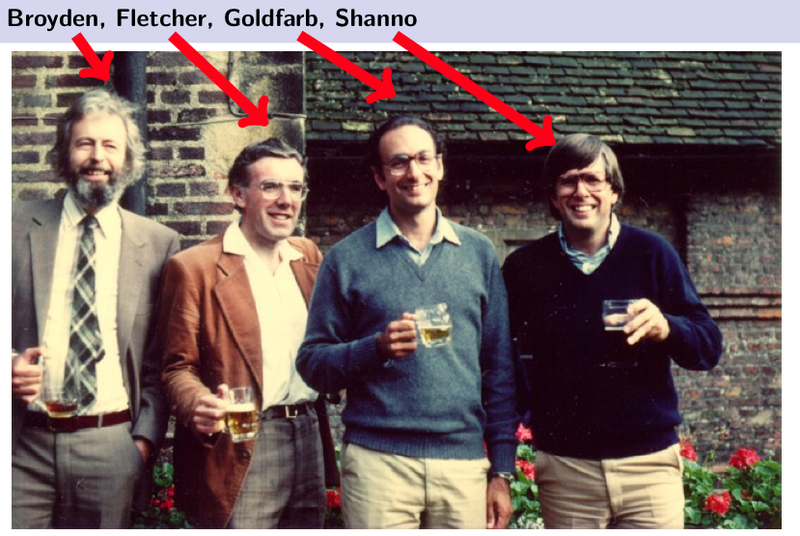
\includegraphics[width=0.6\linewidth]{Images/bfgs.png}
\end{center}
\end{frame}
%%------------Frame 11-----------------------------
\begin{frame}\frametitle{L-BFGS算法(1/3)}
\label{LBFGS_Method}
L-BFGS是Limit-Storage/Limit-Memory BFGS的缩写,其设计的目的就是为了解决BFGS的内存问题(因为$B_k$在数据量较大时候其存储量是非常巨大的),解决的思路就是从下式出发:
\begin{displaymath}
\bm{B}_{k+1}^{-1}=\left(\bm{I}-\frac{\bm{s_ky_{k}^{T}}}{\bm{y_{k}^{T}s_{k}}}\right)\bm{B_k}^{-1}\left(\bm{I}-\frac{\bm{y_ks_{k}^{T}}}{\bm{y_{k}^{T}s_{k}}}\right)+\frac{\bm{s_{k}s_{k}^{T}}}{\bm{y_{k}^{T}s_{k}}}
\end{displaymath}
\begin{itemize}
\item 记$\rho_{k}=\frac{1}{\bm{y_{k}^{T}s_{k}}},\bm{V}_k=\bm{I}-\rho_k\bm{y}_k\bm{s}_k$;
\item 于是有:$\bm{B}_{k+1}^{-1}=\bm{V}_{k}^{T}\bm{B}_{k}\bm{V}_{k}+\rho_{k}\bm{s}_k\bm{s}_{k}^{T}$;递推得到:
\begin{displaymath}
\begin{split}
\bm{B}_{k+1}^{-1}&=\left(\Pi_{i=0}^{k}\bm{V}_{i}^{T}\right)\bm{B}_{0}\left(\Pi_{i=0}^{k}\bm{V}_{i}\right)\\
&+\sum_{j=1}^{k}\left(\left(\Pi_{i=j}^{k}\bm{V}_{i}^{T}\right)(\bm{\rho}_{j-1}\bm{s}_{j-1}\bm{s}_{j-1}^{T})\left(\Pi_{i=j}^{k}\bm{V}_{i}\right)\right)+\rho_{k}\bm{s}_k\bm{s}_{k}^{T}
\end{split}
\end{displaymath}
\end{itemize}
\end{frame}
%%------------Frame 12-----------------------------
\begin{frame}\frametitle{L-BFGS算法(2/3)}
接上一页内容:
\begin{itemize}
\item 计算$\bm{B}_{k+1}$需要$\{\bm{s}_i,\bm{y}_i\}_{k=0}^{k}$,这很耗空间,当$k+1>m$考虑$m$阶截断:
\begin{displaymath}
\begin{split}
\bm{B}_{k+1}^{-1}&=\left(\Pi_{i=k-m+1}^{k}\bm{V}_{i}^{T}\right)\bm{B}_{0}\left(\Pi_{i=k-m+1}^{k}\bm{V}_{i}\right)\\
&+\sum_{j=k-m+2}^{k}\left(\left(\Pi_{i=j}^{k}\bm{V}_{i}^{T}\right)(\bm{\rho}_{j-1}\bm{s}_{j-1}\bm{s}_{j-1}^{T})\left(\Pi_{i=j}^{k}\bm{V}_{i}\right)\right)+\rho_{k}\bm{s}_k\bm{s}_{k}^{T}
\end{split}
\end{displaymath}
\item 通常$m<10$;至此,L-BFGS算法的理论部分就基本完成了,下一节介绍其算法流程。
\end{itemize}
\end{frame}
%%------------Frame 13-----------------------------
\begin{frame}\frametitle{L-BFGS算法(3/3):算法流程\footnote{ Jorge Nocedal.updating quasi-newton matrices with limited storage. Mathematics of Computation.1980.}}
\vspace{-3mm}
\begin{center}
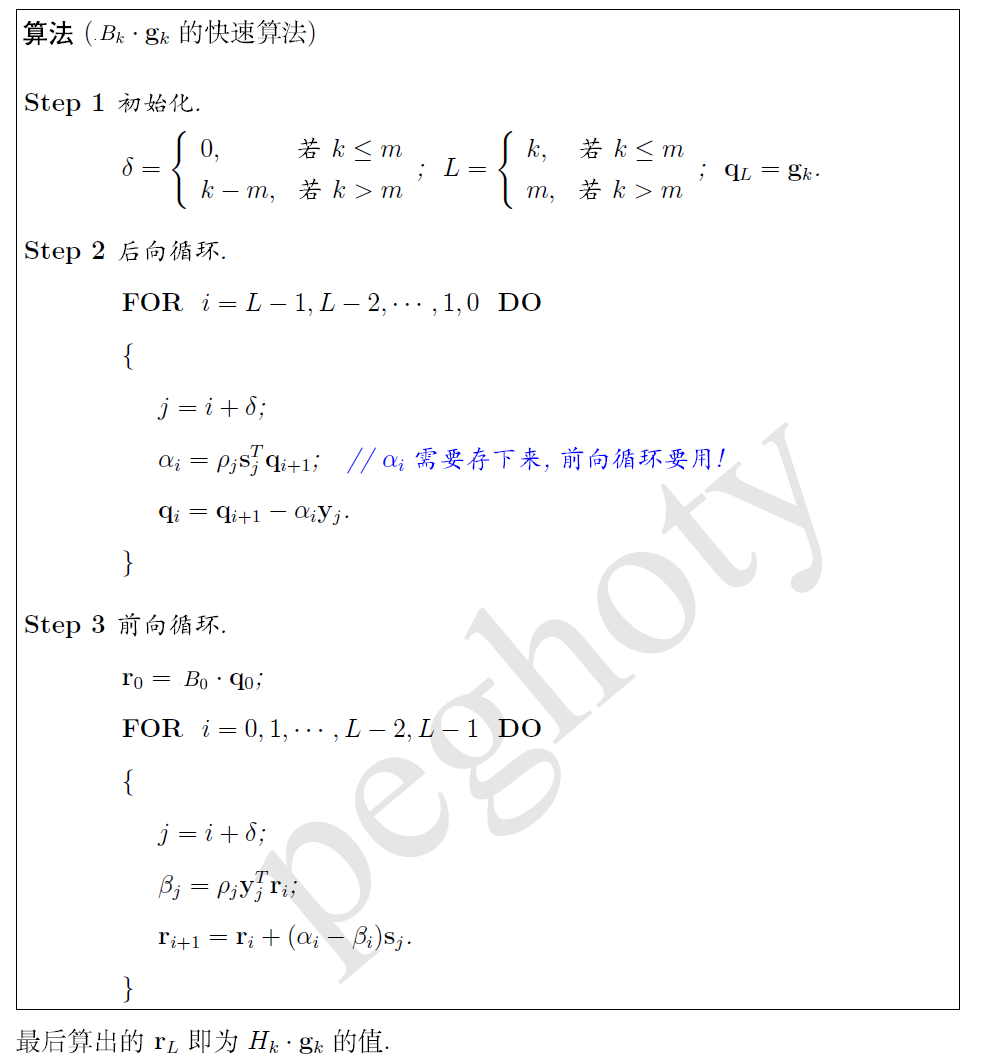
\includegraphics[width=0.54\linewidth]{Images/L-BFGS.png}
\end{center}
\end{frame}
%%------------Frame 14-----------------------------
\begin{frame}\frametitle{次梯度算法(1/3)}
\label{SubGradient_Method}
关于次梯度这里:\url{http://www.hanlongfei.com/convex/2015/10/02/cmu-10725-subgradidient/}做了比较详细的介绍
(这里开始就完全是现学现卖了);首先,来回顾一下凸函数的一阶判别条件\footnote{顺带说一下它的二阶判别条件就是,其Hessian阵是半正定的(如果存在的话)}
\begin{displaymath}
f(\bm{y})\geq f(\bm{x})+\nabla f(\bm{x})^{T}(\bm{y}−\bm{x})
\end{displaymath}
两个条件:1)$f(x)$可微,2)上式在\textbf{整个定义域}都满足

点$x$的\textbf{次梯度}指在函数$f$上的点$x$满足以下条件的$\bm{g} \in \mathbb{R}^{n}$:
\begin{displaymath}
f(\bm{y})\geq f(\bm{x})+\bm{g}^{T}(\bm{y}−\bm{x})
\end{displaymath}
几点注意:
\begin{itemize}
\item $f(x)$可以不是凸函数也不要求它是可微的
\item 该定义是在一个点($x$)上定义的\footnote{个人认为应该还有一定的范围限制,如在$x$的领域内}
\item 次梯度可以有多个(一个集合),可以只有有一个,也可以是空集
\end{itemize}
\end{frame}
%%------------Frame 15-----------------------------
\begin{frame}\frametitle{次梯度算法(2/3)}
几个需要计算次梯度的例子(各个图的函数形式位于图篇的底部):\\
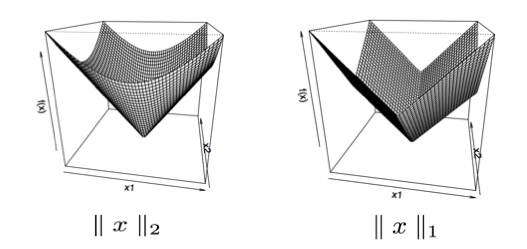
\includegraphics[width=0.5\linewidth]{Images/norm.jpg}
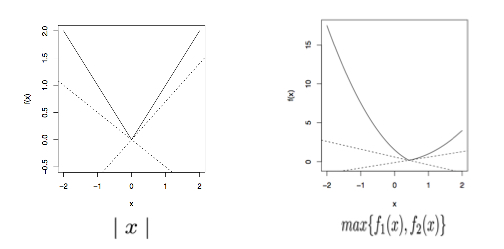
\includegraphics[width=0.5\linewidth]{Images/absolute.jpg}\\
有了次梯度接下来定义次微分(记为$\partial f(\bm{x})$)的概念:
\begin{displaymath}
\partial f(\bm{x})=\{\bm{g} \in \mathbb{R}^{n}: \bm{g}~is~a~subgradient~of~f~at~\bm{x}\}
\end{displaymath}
在第$k$次迭代时有了次梯度$\bm{g}_k \in \partial f(\bm{x})$就可以类似于梯度下降的算法定于次梯度下降算法(其中$t_k$表示步长):
\begin{displaymath}
\bm{x}_{k+1}=\bm{x}_k-t_{k}\bm{g}_k,k=1,2,3,...
\end{displaymath}
\end{frame}
%%------------Frame 16-----------------------------
\begin{frame}\frametitle{次梯度算法(3/3)}
关于次梯度算法,有几点需要注意:
\begin{itemize}
\item 如果目标函数是凸的那么它能保证算法是收敛的,但是次梯度算法并不能保证目标函数每次都是递减的(或者说是单调下降的),为此会有
\begin{displaymath}
f(\bm{x}_{best}^{(k)})=\min_{i=0,1,...,k}\{f(\bm{x}_i)\}=\min\{f(\bm{x}_k),f(\bm{x})_{k-1}\}
\end{displaymath}
\item 当次梯度方向不唯一的时候理论上是选取任意一个都可以的
\item 与梯度下降不同次梯度下降的步长是预先设定好的且满足:
\begin{equation}
\label{Step_Size}
\sum_{i=0}^{\infty}t_i = \infty~and~\sum_{i=0}^{\infty} t_{i}^{2} < \infty
\end{equation}
\end{itemize}
关于公式\ref{Step_Size}最后再说两句:1)公式前半部分保证了搜索范围;2)后半部分保证了步长减小(收敛)
\end{frame}
%%------------Frame 17-----------------------------
\begin{frame}\frametitle{Bregman Projection\footnote{Tsuda, K., Raetsch, G., \& Warmuth, M. K. (2005). Matrix exponentiated gradient updates of online learning and bregman projection. Journal of Machine Learning Research, 6.}(1/2)}
\label{Bregman_Projection}
首先,来回顾一下Bregman Divergence:
\begin{displaymath}
D_{F}(p,q)=F(p)-F(q)-\left<p-q,\nabla F(q)\right>
\end{displaymath}
其中$F(x)$是实值可微的凸函数:$F(x):\Omega \rightarrow R$,而所谓Projection就是指的是将原始空间中的数据(例如下面的$W_1$)投影到某个子空间(集合)的过程。\\
其物理意义就是原数据到这个子空间(集合)的距离最短;所以Bregman  Projection描述的是类似于如下形式的问题:
\begin{displaymath}
\begin{split}
\bm{W}^{*}&=\min_{W} D_F(\bm{W},\bm{W}_1)\\
~~~~s.t~&\bm{W}=\bm{W}^{T},{\rm tr}(\bm{W})=1\\
&{\rm tr}(\bm{W}\bm{C}_j)<0,for~j=1,2,...,n\\
\end{split}
\end{displaymath}
\end{frame}
%%------------Frame 18-----------------------------
\begin{frame}\frametitle{Bregman Projection\footnote{Tsuda, K., Raetsch, G., \& Warmuth, M. K. (2005). Matrix exponentiated gradient updates of online learning and bregman projection. Journal of Machine Learning Research, 6.}(2/2)}
然而全部约束一起考虑太难了,因此Bregman说了:\\
\textit{It is well known that the Bregman projection into the intersection of convex regions can be solved by sequential projections to each region (Bregman, 1967; Censor and Lent,1981)}\\
于是前述问题可以改成每次只考虑一个约束条件的形式(通常是不满足的那个),循环迭代:
\begin{displaymath}
\begin{split}
\bm{W}^{*}&=\min_{W} D_F(\bm{W},\bm{W}_1)\\
~~~~s.t~&\bm{W}=\bm{W}^{T},{\rm tr}(\bm{W})=1\\
&{\rm tr}(\bm{W}\bm{C}_j)\\
\end{split}
\end{displaymath}
\end{frame}
%%------------Frame 19-----------------------------
\begin{frame}\frametitle{Lagrange对偶问题(1/3)}
\label{Lagrange_Dual_Problem}
前面介绍的内容都是目标函数已有后的优化方法,这一部分将会介绍如何将一个一般的有约束的问题转化为Lagrange对偶问题。

原问题:
\begin{equation}
\label{Original_Prob}
\begin{split}
&\min f_0(\bm{x})\\
&s.t~~f_i(\bm{x})\leq 0,i=1,2,...,m\\
&~~~~~h_i(\bm{x}) =0,i=1,2,...,p\\
\end{split}
\end{equation}
Lagrange函数:
\begin{equation}
\label{Lagrange_Func}
\mathcal{L}(\bm{x},\bm{\lambda},\bm{v})=f_0(\bm{x})+\sum_{i=1}^{m}\lambda_i f_i(\bm{x})+\sum_{i=1}^{p}v_ih_i(\bm{x})
\end{equation}
Lagrange对偶函数:
\begin{equation}
\label{Lagrange_Dual}
g(\bm{\lambda},\bm{v})=\inf_{x}\mathcal{L}(\bm{x},\bm{\lambda},\bm{v})=\inf_{x}\left(f_0(\bm{x})+\sum_{i=1}^{m}\lambda_i f_i(\bm{x})+\sum_{i=1}^{p}v_ih_i(\bm{x})\right)
\end{equation}
\end{frame}
%%------------Frame 20-----------------------------
\begin{frame}\frametitle{Lagrange对偶问题(2/3)}
对偶问题\ref{Lagrange_Dual}对任意的$\bm{\lambda} \geq \bm{0}$以及$\bm{v}$都是原问题\ref{Original_Prob}的下界,此外对于$\bm{\lambda} < \bm{0}$的情形这将导致$g(\bm{\lambda},\bm{v})=-\infty$并没有实际意义。

既然$g(\bm{\lambda},\bm{v})$对于任意的$\bm{\lambda} \geq \bm{0}$以及$\bm{v}$是原问题\ref{Original_Prob}的下界,那么什么样的$\bm{\lambda},\bm{v}$才是好的,对偶问题考虑:
\begin{equation}
\label{Dual_Prob}
\max g(\bm{\lambda},\bm{v}),s.t~\bm{\lambda} \geq \bm{0}
\end{equation}
所以实际上的Lagranged对偶问题优化的是:
\begin{displaymath}
\max_{\bm{\lambda},\bm{v}}\left(\min_{\bm{x}}\mathcal{L}(\bm{x},\bm{\lambda},\bm{v})\right)
\end{displaymath}
关于SVM的博客: \url{http://blog.csdn.net/v_july_v/article/details/7624837}\\中把SVM作为一个实例对Lagrange对偶问题进行了解说
\end{frame}
%%------------Frame 21-----------------------------
\begin{frame}\frametitle{Lagrange对偶问题(3/3)}
当原问题是凸问题的时候,满足\textbf{KKT条件}\footnote{KKT:Karush-Kuhn-Tucker}的点也是对偶问题的解。

\textbf{KKT条件:}
\begin{displaymath}
\left\{
\begin{aligned}
&\nabla f_0(\bm{x})+\sum_{i=1}^{m}\lambda_i \nabla f_i(\bm{x})+\sum_{i=1}^{p}v_i \nabla h_i(\bm{x})=\bm{0}\\
&f_i(\bm{x}) \leq 0,i=1,2,...,m\\
&h_i(\bm{x}) =0,i=1,2,...,p\\
&\lambda_i \geq 0,i=1,2,...,m\\
&\lambda_i f_i(\bm{x})=0, i=1,2,...,m\\
\end{aligned}
\right.
\end{displaymath}
\end{frame}
%%------------Frame 22-----------------------------
\begin{frame}\frametitle{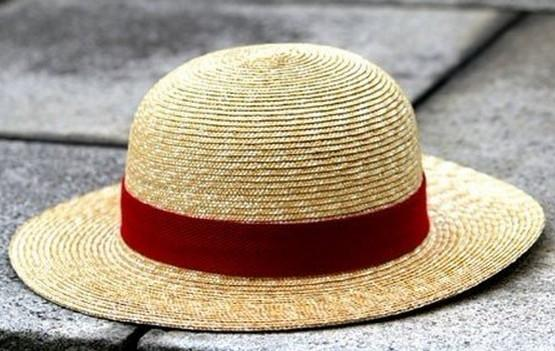
\includegraphics[width=7mm,height=5mm]{Images/strawhat.jpg}几个例子——之一(1/4)}
\label{Examples}
首先,第一个例子来介绍一下Mexico草帽:\\
\begin{center}
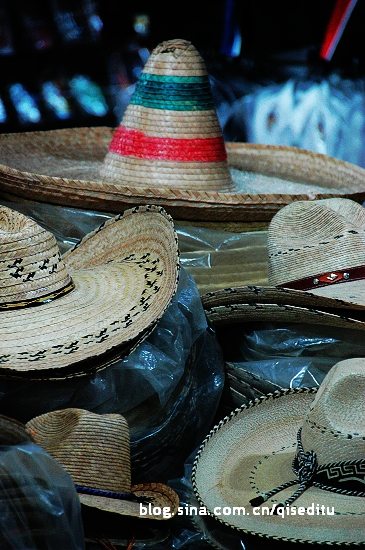
\includegraphics[width=0.2\linewidth , height=0.4\linewidth]{Images/mexicohat.jpg}
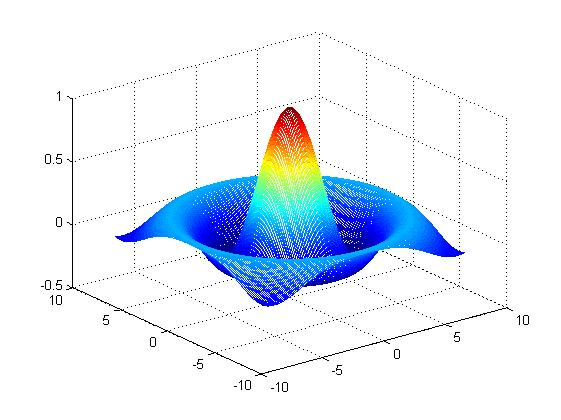
\includegraphics[width=0.4\linewidth]{Images/opthat.jpg}
\end{center}
函数的形式:$f(x,y)=\frac{\sin(\sqrt{x^2+y^2})}{\sqrt{x^2+y^2}}$
\end{frame}
%%------------Frame 23-----------------------------
\begin{frame}\frametitle{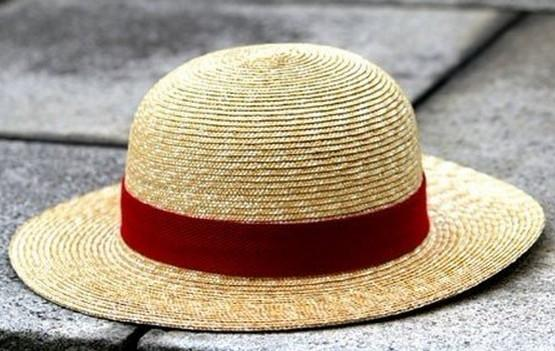
\includegraphics[width=7mm,height=5mm]{Images/strawhat.jpg}几个例子——之一(2/4)}
{\tiny
接上一页:
\begin{itemize}
\item 函数的梯度形式:
\begin{displaymath}
\partial f(x,y)=\left\{
\begin{split}
&\cos(\sqrt{x^2+y^2})\frac{x}{x^2+y^2}-\sin(\sqrt{x^2+y^2})\frac{x}{\sqrt{x^2+y^2}^3}\\
&\cos(\sqrt{x^2+y^2})\frac{y}{x^2+y^2}-\sin(\sqrt{x^2+y^2})\frac{y}{\sqrt{x^2+y^2}^3}\\
\end{split}
\right.
\end{displaymath}
\item Hessian 矩阵:
\begin{displaymath}
H=\left[
\begin{array}{cc}
a_{11}&a_{12}\\
a_{12}&a_{22}\\
\end{array}
\right]~where~
\left\{
\begin{split}
&a_{11}=-\sin(\sqrt{x^2+y^2})\frac{x^2(x^2+y^2)+y^2-2x^2}{\sqrt{x^2+y^2}^5}\\
&~~~~~~~+\cos(\sqrt{x^2+y^2})\frac{(y^2-2x^2)}{\sqrt{x^2+y^2}^4}\\
&a_{12}=-\sin(\sqrt{x^2+y^2})\frac{xy(x^2+y^2)-3xy}{\sqrt{x^2+y^2}^5}\\
&~~~~~~~-\cos(\sqrt{x^2+y^2})\frac{3xy}{\sqrt{x^2+y^2}^4}\\
&a_{22}=-\sin(\sqrt{x^2+y^2})\frac{y^2(x^2+y^2)+x^2-2y^2}{\sqrt{x^2+y^2}^5}\\
&~~~~~~~+\cos(\sqrt{x^2+y^2})\frac{(x^2-2y^2)}{\sqrt{x^2+y^2}^4}\\
\end{split}
\right.
\end{displaymath}
\end{itemize}
}
\end{frame}
%%------------Frame 24-----------------------------
\begin{frame}
\frametitle{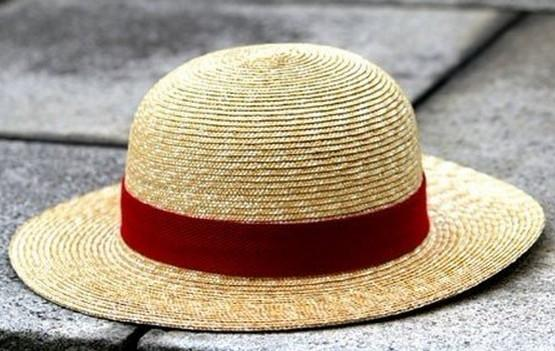
\includegraphics[width=7mm,height=5mm]{Images/strawhat.jpg}几个例子——之一(3/4)}
首先注意到的是:即便是如此简单的一个函数函数其Hessian矩阵也是难以计算的。\\
下面就来看一下墨西哥草帽上的优化问题的一些结果:
\vspace{-3mm}
\begin{table}[h]
\centering
\begin{tabular}{|c|c|c|c|c|c|}\hline
\multicolumn{6}{|c|}{Mexico\_hat(range=[-10,10,-10,10],step=0.2,scale=101$\times$101)} \\\hline
算法 &总时间(单位:s) &maxiter &average\_iter &存储 &备注\\ \hline
grad &8.450431 &500 &93.97 &$O(n)$ &\#\#\#\\ \hline
newton &3.720508 &500 &5.43 &$O(n^2)$ &\#\#\#\\ \hline
bfgs &14.776714 &500 &42.27 &$O(n^2)$ &\#\#\#\\ \hline
\end{tabular}
%\caption{}
\label{exp_1}
\end{table}
\end{frame}
%%------------Frame 25-----------------------------
\begin{frame}
\frametitle{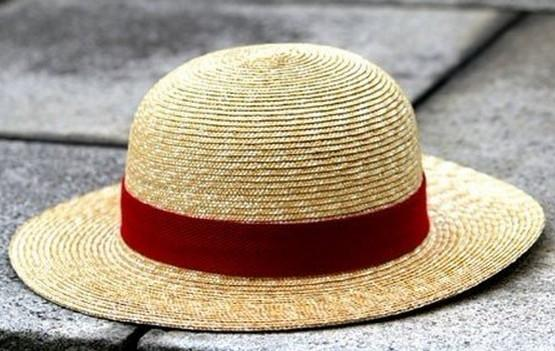
\includegraphics[width=7mm,height=5mm]{Images/strawhat.jpg}几个例子——之一(4/4)}
再来看几张图(从左到右:grad->newton->bfgs):\\
\vspace{-3mm}
\begin{center}
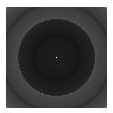
\includegraphics[width=0.23\linewidth]{Images/grad_hat.jpg}
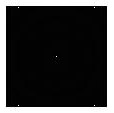
\includegraphics[width=0.23\linewidth]{Images/newton_hat.jpg}
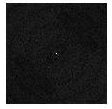
\includegraphics[width=0.23\linewidth]{Images/bfgs_hat.jpg}
\end{center}
\vspace{-3mm}
把图片稍微锐化一下就是下面的样子了:\\
\vspace{-3mm}
\begin{center}
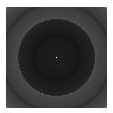
\includegraphics[width=0.23\linewidth]{Images/grad_hat.jpg}
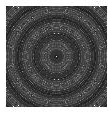
\includegraphics[width=0.23\linewidth]{Images/newton_hat_20.jpg}
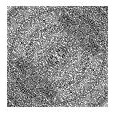
\includegraphics[width=0.23\linewidth]{Images/bfgs_hat_80.jpg}
\end{center}
\vspace{-3mm}
这些图片代表了在[-10,10,-10,10]的范围内以0.2为步长遍历所有点,并把它作为初始值赋给算法,然后各个点的灰度值代表了迭代次数大小
\end{frame}
%%------------Frame 26-----------------------------
\begin{frame}
\frametitle{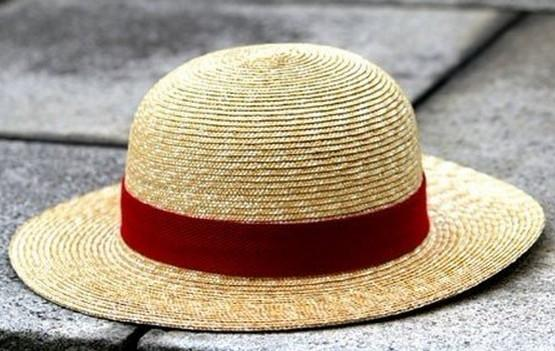
\includegraphics[width=7mm,height=5mm]{Images/strawhat.jpg}几个例子——之二(1/2)}
这次做的是回归问题:$f(x)=p_1e^{p_2x}$,采样$x=-1:0.02:1$,获得观测值$yn=f(x)$,其中真实参数$(p_1,p_2)=(0.5,0.1)$,目标函数:
\begin{displaymath}
\min\|\epsilon\epsilon^{T}\|,\epsilon=\hat{y}-yn
\end{displaymath}
这次直接上结果:\\
\vspace{-3mm}
\begin{table}[h]
\centering
\begin{tabular}{|c|c|c|c|c|c|}\hline
\multicolumn{6}{|c|}{fit(range=[-1,1,-1,1],step=0.02,scale=101$\times$101)} \\\hline
算法 &总时间(单位:s) &maxiter &average\_iter &存储 &备注\\ \hline
grad &90.776934 &178 &156.14 &$O(ns)$ &\#\#\# \\ \hline
levmar &160.395254 &384 &351.70 &$O(ns)$ &$\mu=1$ \\ \hline
levmar &91.96887 &217 &200.64 &$O(ns)$ &$\mu=0.1$ \\ \hline
levmar &84.676262 &200 &185.18 &$O(ns)$ &$\mu=0.01$ \\ \hline
levmar &83.078666 &198 &182.28 &$O(ns)$ &$\mu=0$ \\ \hline
\multicolumn{6}{|c|}{fit(range=[-10,10,-10,10],step=0.02,scale=1001$\times$1001)} \\\hline
grad &14965.815 &500 &332.04 &$O(ns)$ &\#\#\# \\ \hline
levmar &31156.32704 &500 &486.58 &$O(ns)$ &$\mu=0$ \\ \hline
\end{tabular}
%\caption{}
\label{exp_2}
\end{table}
\end{frame}
%%------------Frame 27-----------------------------
\begin{frame}
\frametitle{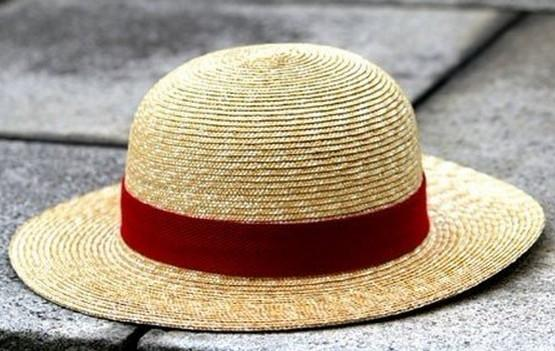
\includegraphics[width=7mm,height=5mm]{Images/strawhat.jpg}几个例子——之二(2/2)}
\vspace{-1mm}
最后还是看几个图(从左到右:grad,levmar($\mu=0.01$),levmar($\mu=1$)):\\
\vspace{-1mm}
{\centering
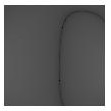
\includegraphics[width=0.2\linewidth]{Images/fit_grad_small.jpg}

\includegraphics[width=0.21\linewidth]{Images/fit_levmar_0.01.jpg}
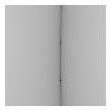
\includegraphics[width=0.205\linewidth]{Images/fit_levmar_1.jpg}\\
}
\vspace{-1mm}
更大范围内的情况(range=[-10,10,-10,10],左到右:grad,levmar($\mu=0$)):\\
\vspace{-1mm}
\begin{center}
\fbox{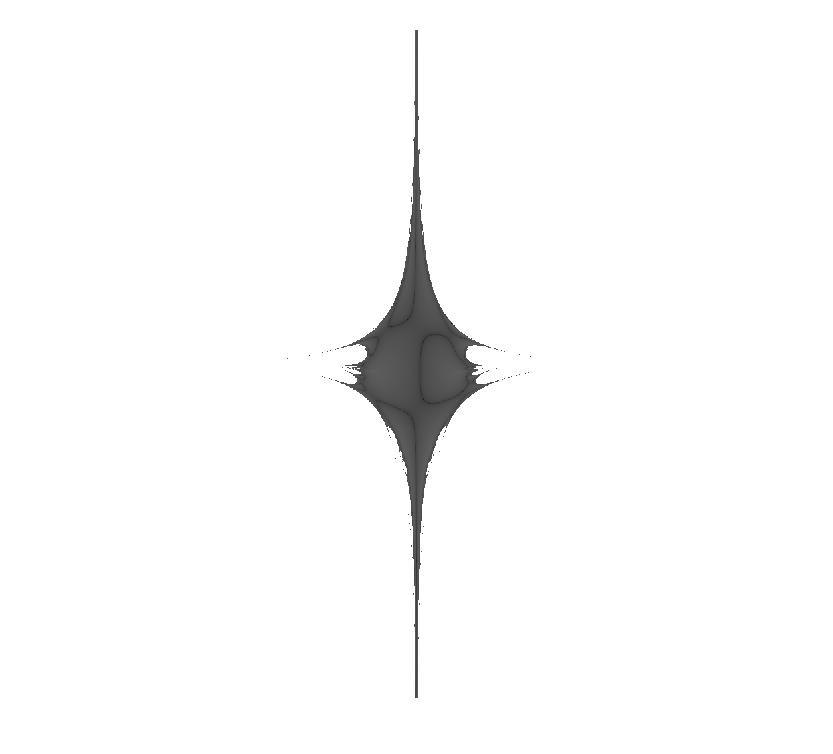
\includegraphics[width=0.4\linewidth]{Images/fit_grad.jpg}}
\fbox{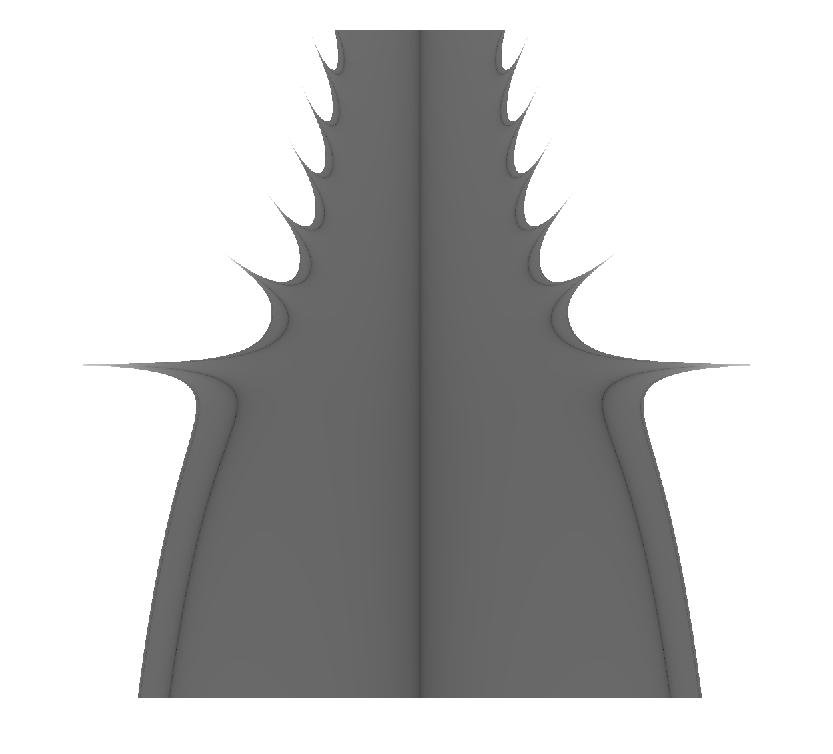
\includegraphics[width=0.4\linewidth]{Images/fit_levmar.jpg}}
\end{center}
\end{frame}
%%------------Frame 27-----------------------------
\begin{frame}
\frametitle{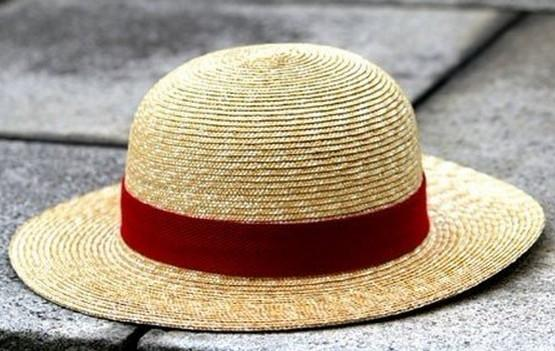
\includegraphics[width=7mm,height=5mm]{Images/strawhat.jpg}几个例子——之Newton法与多项式($x^3-0.01$)}
\vspace{-3mm}
\begin{center}
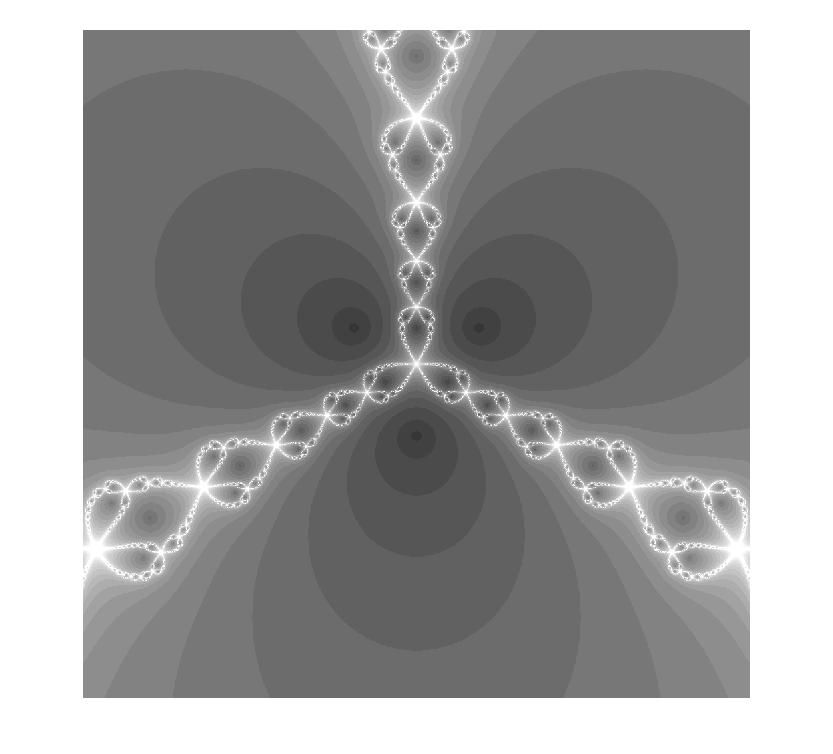
\includegraphics[width=0.9\linewidth]{Images/newton_poly_3.jpg}
\end{center}
\end{frame}
%%------------Frame 28-----------------------------
\begin{frame}
\frametitle{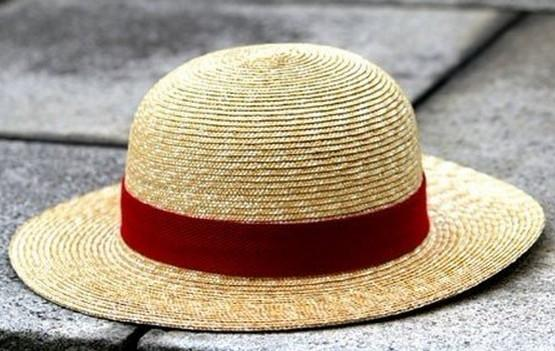
\includegraphics[width=7mm,height=5mm]{Images/strawhat.jpg}几个例子——之Newton法与多项式($x^6-0.01$)}
\vspace{-3mm}
\begin{center}
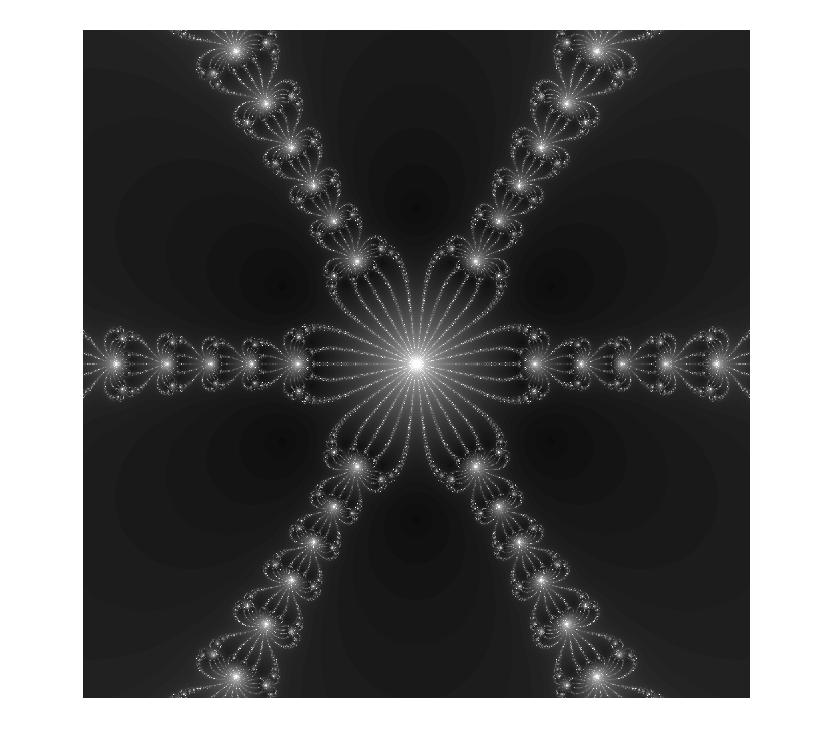
\includegraphics[width=0.85\linewidth]{Images/newton_poly_6.jpg}
\end{center}
\end{frame}
%%------------Frame 29-----------------------------
\begin{frame}
\frametitle{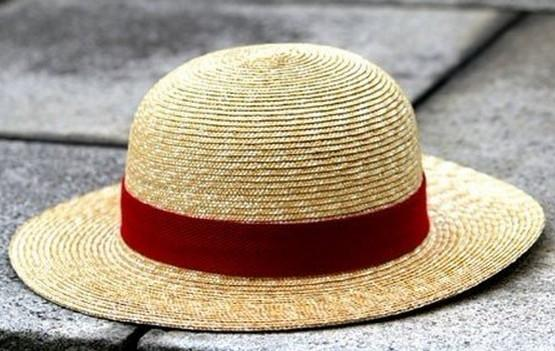
\includegraphics[width=7mm,height=5mm]{Images/strawhat.jpg}几个例子——之Newton法与多项式($x^{13}-0.01$)}
\vspace{-3mm}
\begin{center}
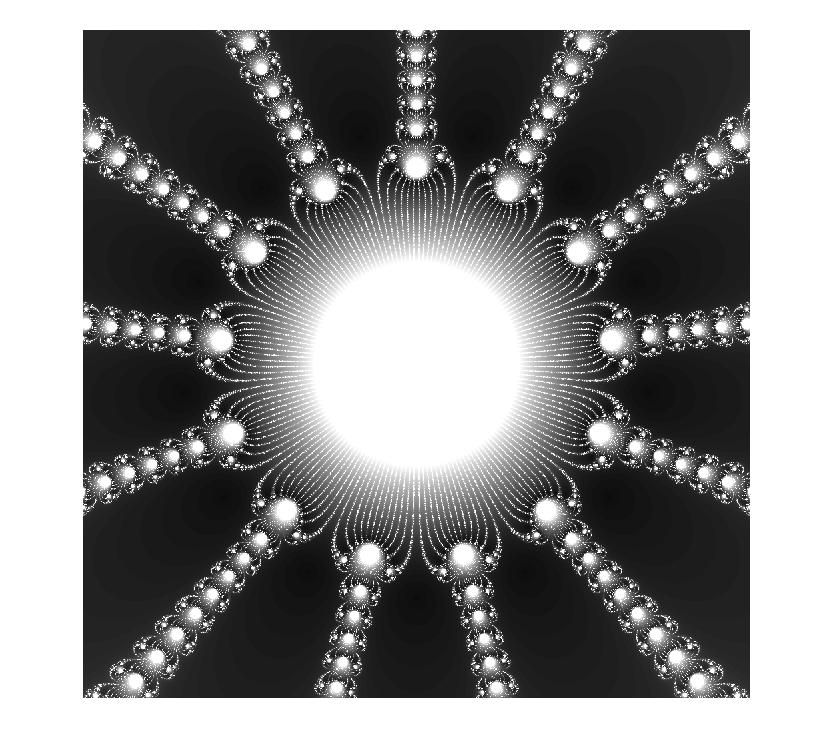
\includegraphics[width=0.8\linewidth]{Images/newton_poly_13.jpg}
\end{center}
\end{frame}
\begin{frame}\frametitle{下集预告}
\label{Next}
\begin{itemize}
\item 本集遗漏的内容
\begin{itemize}
\item 共轭梯度算法
\item EM算法
\end{itemize}
\item 一维搜索(线搜),以下内容全凭记忆想到,欢迎指正和补充
\begin{itemize}
\item 二分查找
\item 0.618法
\item BFGS一维的情况
\item 其它(暂时没想好)
\end{itemize}
\end{itemize}
\end{frame}
%%------------Frame 30-----------------------------
\begin{frame}\frametitle{Q\&A \tiny{由于是现学现卖,我尽力而为}}
\label{Q_and_A}
\begin{center}
\huge{谢谢!}
\end{center}
\end{frame}
%%------------Document end-----------------------------
\end{document}